\documentclass[11pt,a4paper]{article}
\usepackage[utf8]{inputenc}
\usepackage[T1]{fontenc}
\usepackage[english]{babel}
\usepackage[margin=2.1cm]{geometry}
\usepackage{booktabs,array,tabularx}
\usepackage{xcolor}
\usepackage{graphicx}
\usepackage{pgfplots}
\pgfplotsset{compat=1.17}
\PassOptionsToPackage{hyphens}{url}
\usepackage[hidelinks]{hyperref}
\usepackage{enumitem}
\setlist{nosep,leftmargin=1.4em}
\emergencystretch=3em

\definecolor{impl}{HTML}{3B6EA8}
\definecolor{rev}{HTML}{8FB3DA}
\definecolor{waste}{HTML}{C0504D}

\title{Sweatshop on P-Chess: lane \texttt{core}, afternoon\\\large The UCI bridge, a game against Maia and the clocks (BOT-002, BOT-004, CLOCK-001); Opus 5.5 lineup}
\author{Foreman, session \texttt{sweatshop/core/2026-10-24-1535}}
\date{24 October 2026}

\begin{document}
\maketitle

\section*{Summary}

Lane \texttt{core} ran in the clone \path{.artifacts-build/lanes/core}, from \texttt{main} at
\texttt{7813c75} (PR \#5 merged, so BOT-001 and its engine fetch script were on the base).
Every open ticket of the three lanes waited on one chain here: BOT-002 $\rightarrow$ BOT-004
$\rightarrow$ CLOCK-001. Two launches, both with \texttt{-Models 'stage 2 opus-5.5 high, hard
opus-5.5 xhigh, stage 3 opus-5.5 xhigh'} (Bruno's choice; the same models as the
\texttt{night} binding, logged by the driver as \texttt{ad hoc}): 15:35 (pid 18936, ended 16:11
``Nothing runnable'' after the driver parked a valid BOT-004 handoff) and 16:12 (pid 9808,
stopped with \texttt{STOP} at 17:55, once CLOCK-001 was merged, as the supervising session
asked). Before launch the foreman fetched \path{engine/} into the clone with
\path{scripts/fetch-engine.ps1} (every hash verified, gitignored), so the live Lc0 tests ran
instead of being skipped.

\begin{itemize}
  \item \textbf{Produced:} \textbf{3 tickets approved and merged on the session} PR
        \href{https://github.com/Laginho/P-Chess/pull/6}{\#6}: BOT-002, BOT-004, CLOCK-001,
        all \texttt{Review: agent}, \texttt{Verdict: Approve}, no \emph{Needs your call}.
        BOT-004 and CLOCK-001 close with \texttt{Acceptance: pending} (manual checks, release
        impact).
  \item \textbf{Cost:} \textbf{\$24.89} at API list price over 8 stages, all priced:
        \texttt{opus-5.5 xhigh} \$17.09 (hard stage 2 and every review),
        \texttt{opus-5.5 high} \$7.79. No Codex model ran a stage (Codex quota: \texttt{--});
        one \texttt{gpt-6-astra medium} call judged the reopen (section Reopen attribution).
  \item \textbf{What went wrong:} BOT-004's 50~ms latency criterion. The first review
        measured 74--106~ms in the windowed app and reopened; the retry found the machine
        saturated by three lanes and another project (Lc0 alone 247--813~ms per move). The
        proxy turned the target into manual acceptance and Bruno deferred the measurement to
        an idle machine. The reopen cost \$4.54 (review plus retry).
  \item \textbf{Provisional verdict:} Opus 5.5 high implementing under Opus 5.5 xhigh review
        delivered the chain in 2h20 with one reopen, whose cause was the environment more
        than the code. The live engine paid for itself at once: it found a real shutdown bug
        in BOT-002 that the rebuilt fixture had hidden.
\end{itemize}

\section*{What was done}

\textbf{BOT-002}: the game can now talk to Lc0. \path{engine/uci.gd} starts Lc0 once, reads
it on worker threads, switches Maia nets, and returns Maia's policy (a probability per legal
move) on the main thread. The reviewed work of the night run was cherry-picked (its merge had
been reverted for want of BOT-001), and this time the parser's fixture was recorded from the
real Lc0 v0.32.1 and the level-switch test ran live. The live run caught a bug: the reader
threads ran a method of the bridge node, which in debug builds locked the node, so
\texttt{free()} failed and Lc0 was never stopped; the method became \texttt{static}. The
recording also settled that Lc0's default \texttt{PolicyTemperature} is 1.359.

\textbf{BOT-004}: a player can pick a colour and a Maia level (1100--1900) on a new setup
screen and play a full game against her. \path{bot/maia_player.gd} drops illegal policy
entries, samples with BOT-003's move picker, and logs Maia's reply latency, printing the
median at game end; the board ignores input while Maia is to move. Reopened once: criterion 4
(median under 50~ms) failed in the windowed app with a human-like pause (74.4 and 105.5~ms),
with the machine under heavy load. Not an implementation fix: the proxy rewrote criterion 4 to
``record and print the median'' and Bruno deferred the 50~ms check to an idle machine.

\textbf{CLOCK-001}: games are timed. \path{core/clock.gd} counts milliseconds, leaves each
side's first move untimed and without increment (as Lichess does), plays the low-time warning
once, and flags at zero; the setup screen offers 1+0, 3+2 and 5+0, and a flag ends the game
through CORE-004's rule. A proxy decision added criterion 8 and \path{ui/board_view.gd}: a
piece dropped after the game ended snaps back instead of adding a move. The review's three
mutants each failed their own test.

\section*{Timeline}

\begin{tabularx}{\linewidth}{@{}lX@{}}
\toprule
15:35 & Clone pulled to \texttt{7813c75}; \path{engine/} fetched. Session opened locally (\texttt{43fe465}); BOT-002 restored to \texttt{to-implement} (\texttt{c99686f}), old branch kept as \texttt{recovery/20261024-153504/BOT-002}. Launch, pid 18936. \\
15:47 & BOT-002 implement (hard): to review, fixture recorded, c7 live, 86/0. \\
15:56 & BOT-002 review: merged (\texttt{5143b81}). \\
16:10 & BOT-004 implement: valid handoff (92/0) parked as ``missing Gate evidence receipt''. \\
16:11 & Driver ends; PR \#6 opened. \\
16:14 & Foreman: receipt line fixed on the ticket branch, park \texttt{d44ea41} reverted (\texttt{1f45929}). Relaunch, pid 9808. \\
16:28 & BOT-004 review: reopened, criterion 4. \\
16:45 & Bruno (relayed): defer the latency check to an idle machine; recorded on the session (\texttt{3777aad}). \\
16:53 & BOT-004 retry: to review, no code change, criterion 4 rewritten by the proxy. \\
17:12 & BOT-004 review: merged (\texttt{34e432c}). \\
17:41 & CLOCK-001 implement: to review, 102/0. \texttt{STOP} created as the review starts. \\
17:55 & CLOCK-001 review: merged (\texttt{c160ef0}); driver stops; PR \#6 updated (3 tickets). \\
\bottomrule
\end{tabularx}

\section*{Per stage}

{\small
\begin{tabularx}{\linewidth}{@{}llllrrrrrX@{}}
\toprule
When & Ticket & Stage & Model & Min & In & Cache & Out & Cost & Outcome \\
\midrule
15:47 & BOT-002 & impl & opus xhigh & 12 & 7.7M & 97\% & 52k & 3.94 & to-review \\
15:56 & BOT-002 & review & opus xhigh & 9 & 2.7M & 95\% & 47k & 1.68 & merged \\
16:10 & BOT-004 & impl & opus high & 14 & 4.5M & 98\% & 38k & 2.44 & to-review$^{*}$ \\
16:28 & BOT-004 & review & opus xhigh & 15 & 4.5M & 96\% & 52k & 2.40 & reopened \\
16:53 & BOT-004 & impl & opus high & 23 & 3.4M & 96\% & 33k & 2.14 & to-review \\
17:12 & BOT-004 & review & opus xhigh & 19 & 11.3M & 98\% & 86k & 5.65 & merged \\
17:41 & CLOCK-001 & impl & opus high & 29 & 5.9M & 97\% & 47k & 3.21 & to-review \\
17:55 & CLOCK-001 & review & opus xhigh & 13 & 6.4M & 96\% & 72k & 3.44 & merged \\
\midrule
 & & & & 134 & 46.4M & & 427k & 24.89 & \\
\bottomrule
\end{tabularx}
}

\smallskip
{\small $^{*}$ The run-log row reads \texttt{failed (incomplete handoff), blocked}. The handoff
was valid; the driver did not read its receipt line (Driver issues, 1). The row is left as
logged.}

\begin{center}
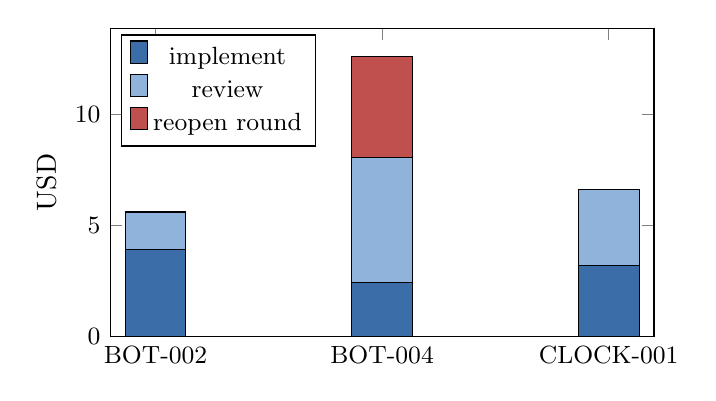
\begin{tikzpicture}
\begin{axis}[ybar stacked, bar width=22pt, width=0.7\linewidth, height=5.5cm,
  symbolic x coords={BOT-002,BOT-004,CLOCK-001},
  xtick=data, ylabel={USD}, ymin=0, legend style={at={(0.02,0.98)},anchor=north west,font=\small},
  tick label style={font=\small}]
\addplot[fill=impl] coordinates {(BOT-002,3.94) (BOT-004,2.44) (CLOCK-001,3.21)};
\addplot[fill=rev] coordinates {(BOT-002,1.68) (BOT-004,5.65) (CLOCK-001,3.44)};
\addplot[fill=waste] coordinates {(BOT-002,0) (BOT-004,4.54) (CLOCK-001,0)};
\legend{implement, review, reopen round}
\end{axis}
\end{tikzpicture}
\end{center}

The red segment is BOT-004's first review and its retry (\$4.54), spent on a criterion the
machine could not measure. BOT-004's closing review was the costliest stage (11.3M input,
\$5.65): it resolved four rebase conflicts with Bruno's deferral, moved BOT-002's open notes to
other tickets and rebuilt a gate receipt by hand. Input is 95--98\% cache reads.

\section*{Comparison with previous runs}

From \texttt{run-log.md}: the night \texttt{core} run, same lineup family, cost \$7.20 per
approved ticket; lane \texttt{mvp} \$2.69 (small tickets, day lineup); this run \$8.30
(\$24.89 over 3). These were the heaviest tickets so far (a process bridge with threads, a
first playable bot screen, a clock wired through the UI), and BOT-004 alone is 54\% of the
cost. Stage 2 took 12--29~min here (median 18.5) against a 6~min median for 	exttt{opus-5.5 high} overall.

\section*{Observations per model}

\begin{itemize}
  \item \textbf{opus-5.5 xhigh, hard stage 2 (BOT-002)}: reused the reviewed work as told,
        recorded the fixture from the live engine, and found the shutdown bug from a failing
        live test, with the before and after kept as proof.
  \item \textbf{opus-5.5 high, stage 2 (BOT-004 twice, CLOCK-001)}: every handoff disclosed
        what it had not checked (manual games, drag smoothness, the one-frame flag race). On
        the BOT-004 retry it measured, found the machine saturated, and asked the proxy
        instead of tuning \path{engine/uci.gd} outside its files. Its first BOT-004 handoff
        wrote the receipt line as a bullet with a note, which the driver cannot read.
  \item \textbf{opus-5.5 xhigh, review}: three merges and one reopen; no code authored in
        review, so no round-0 rows. It measured criterion 4 in the real windowed app rather
        than trusting the headless test, ran mutants on CLOCK-001, and turned every open note
        into a ticket or a destination (BOT-008, CLOCK-002, notes on BOT-005, BOT-007,
        HIST-002). Two habits cost elsewhere: notes written into other lanes' tickets, and a
        gate receipt written by hand when the helper was denied.
\end{itemize}

\section*{Driver and runtime issues}

\begin{enumerate}
  \item \textbf{\texttt{- Gate evidence:} is invisible to the driver.} \texttt{Field()} only
        reads a line that starts with \texttt{Gate evidence:}; a bullet, or a trailing note
        after the path, parks a valid handoff. Fourth time today (CORE-001, CORE-005 in the
        night run, BOT-004 here). It also mischarges the scoreboard: the next review is
        attributed to implementer \texttt{?}.
  \item \textbf{\texttt{gate-evidence.ps1} denied in stage sessions.} BOT-002's stage 2 got it
        through only in one exact Bash form (a proxy decision); BOT-004's review could not run
        it and wrote the receipt by hand from a manual gate run. The receipt matched, but a
        hand-written receipt is not the evidence the check was built for.
  \item \textbf{A merged-and-reverted branch cannot be re-reviewed.} BOT-002's commits were
        ancestors of \texttt{main} through the reverted merge, so restoring
        \texttt{to-review} would have merged nothing. The foreman restored
        \texttt{to-implement} with a cherry-pick instruction and quoted the stale record so
        the driver would not read its old receipt, verdict and acceptance lines.
  \item \textbf{Shared machine.} A latency criterion ran with three lanes and another project
        on the same PC; neither the driver nor the stage can tell code cost from load.
\end{enumerate}

\section*{Recommendations}

\begin{enumerate}
  \item Make the driver's \texttt{Field()} accept an optional leading \texttt{- } and stop at
        whitespace after a path, or have ticket-flow's handoff template show the exact line.
        Rests on four parked handoffs today; scoreboard row \texttt{?} $\rightarrow$
        \texttt{opus-5.5 xhigh} (3 reviews) exists only because of it.
  \item Allow the gate helper's command form in the stage sessions' permissions (Bruno's
        call), so no review writes a receipt by hand.
  \item Write timing criteria as manual acceptance on an idle machine from the start, or run
        them only when no other lane runs. BOT-004's reopen round cost \$4.54.
  \item In ticket-flow, route a review's notes for another lane's ticket to its own ticket or
        the base, not into the other lane's folder: BOT-005 and BOT-007 will conflict when
        the bot and mvp lanes sync.
  \item Keep \texttt{opus-5.5 high} $\rightarrow$ \texttt{opus-5.5 xhigh} for the core chain:
        8 reviews, 2 reopened, S2 rate 25\% (an anecdote under 10 reviews), plus BOT-004's
        reopen mischarged to \texttt{?}.
\end{enumerate}

\section*{Human debt and proxy decisions}

No \texttt{Débito humano:} lines this run. Bruno decided twice, relayed by the supervising
session: unblock BOT-002 after BOT-001 merged; defer BOT-004's latency measurement until the
machine is idle (``deixa a parte do tempo de resposta pra depois''). \texttt{Proxy decided}
lines, all \texttt{(opus)}, spawned by the stages:

\begin{itemize}
  \item \textbf{BOT-002}: retry \texttt{gate-evidence.ps1} once as a single
        \texttt{powershell -NoProfile -File} Bash command; never hand in work without a
        receipt. (The night run's option A, a rebuilt fixture, is superseded by the
        recording.)
  \item \textbf{BOT-004}: criterion 4 keeps the 50~ms target as M3 product acceptance,
        measured in a manual game on an idle machine; the loop checks only that latency is
        recorded and its median logged; \path{engine/uci.gd} stays out of Primary files.
  \item \textbf{BOT-004}: \texttt{PolicyTemperature} stays Bruno's question, carried by notes
        on BOT-005 and BOT-007; the missing Lc0-stop detection becomes ticket BOT-008.
  \item \textbf{BOT-004}: hand-run the gate helper's steps for a fresh receipt on
        \texttt{0ad3d14}, the helper being denied by permissions.
  \item \textbf{CLOCK-001}: a side's first move is untimed and adds no increment, as on
        Lichess (criterion 2).
  \item \textbf{CLOCK-001}: \path{ui/board_view.gd} (\texttt{\_commit}) and its test join
        Primary files with criterion 8; a drop after the game ends snaps back.
\end{itemize}

\section*{Reopen attribution}

One reopened review; judged by \texttt{gpt-6-astra medium}, read-only, since the reviewer is
Opus. No merging review authored a fix, so no round-0 rows. PR \#6 has no review findings yet;
no session-review, release-audit or post-release discovery.

{\small
\noindent\begin{tabularx}{\linewidth}{@{}lcXp{2.4cm}X@{}}
\toprule
Ticket & Rnd & Finding & Label & Why \\
\midrule
BOT-004 & 1 & Windowed median 74.4 / 105.5~ms against criterion 4's 50~ms & S2-explícito/\allowbreak código & The original criterion explicitly requires under 50~ms; the measurements do not isolate code cost from machine load. Review miss: no. Churn: no. \\
\bottomrule
\end{tabularx}
}

\smallskip
Totals: S2-explícito/código 1. The foreman notes that the cause was most likely load, not
code (the retry measured Lc0 alone at 247--813~ms), and that the criterion was later rewritten
by the proxy; the label stands as returned. The scoreboard charges this round to \texttt{?},
not to \texttt{opus-5.5 high} (Driver issues, 1).

\section*{Scoreboard}

\texttt{scoreboard.ps1} over P-Chess (main checkout, log merged and copied back), ClassyCall,
EasyMath, PhysiSyst, SIGAA-ME, SynchroNice and slip. Rows that moved since the \texttt{mvp}
report: \texttt{opus-5.5 high} $\rightarrow$ \texttt{opus-5.5 xhigh} 6 $\rightarrow$ 8
reviews, still 2 reopened (33\% $\rightarrow$ 25\%); \texttt{opus-5.5 xhigh} $\rightarrow$
\texttt{opus-5.5 xhigh} 5 $\rightarrow$ 7, 0 reopened; a new row \texttt{?} $\rightarrow$
\texttt{opus-5.5 xhigh} 3 reviews, 1 reopened, 1 unclassified (BOT-004's round, mischarged).
All Opus pairs remain under 10 reviews: anecdotes. The attribution and intervention rows of
this run are committed on \texttt{main} with this report; the printout was taken from the
main checkout before that commit, so they are not in it.

{\small
\begin{tabular}{@{}llrrrrr@{}}
\toprule
Implementer & Reviewer & Reviews & Reopened & Rate & S2 & S2 rate \\
\midrule
gpt-6.1-sol high & gpt-6.1-sol xhigh & 89 & 12 & 13\% & 11 & 12\% \\
gpt-6.1-sol high & gpt-6.1-sol max & 94 & 21 & 22\% & 20 & 21\% \\
opus-5.5 high & opus-5.5 xhigh & 8 & 2 & 25\% & 2 & 25\% \\
opus-5.5 xhigh & opus-5.5 xhigh & 7 & 0 & 0\% & 0 & 0\% \\
? & opus-5.5 xhigh & 3 & 1 & 33\% & 0 & $\geq$0\% \\
sonnet-5.5 high & opus-5.5 xhigh & 3 & 0 & 0\% & 0 & 0\% \\
\bottomrule
\end{tabular}
}

\medskip
Implementers: \texttt{opus-5.5 high} 14 runs, 10 to review, 4 failed, median 6~min, \$24.96;
\texttt{opus-5.5 xhigh} 19 runs, 14 to review, 5 failed, median 12~min, \$90.74. Interventions
across repos: 22 human rescues, 48 automatic recoveries, 6 routine approvals, 30
\texttt{gpt-6-astra high, fallback}, 15 Opus and 12 supervisor proxy decisions, 37 unknown.
Runtime completion to process exit: 854~s over 609 measured stages, 756 unmeasured. Full
printout: the foreman's scratch output.

\section*{Pending for the human}

\begin{enumerate}
  \item Merge PR \#6 (BOT-002, BOT-004, CLOCK-001); then the bot lane (BOT-005, BOT-006) and
        later mvp (BOT-007, CI-002) can start, and the other open lanes sync.
  \item BOT-004: measure Maia's latency with the machine idle (a windowed game against
        maia-1500 as each colour; median under 50~ms). Over 50~ms: a ticket with
        \path{engine/uci.gd} in Primary files for Lc0's thread options.
  \item CLOCK-001: lose a 1+0 game on time; win a game on time against Maia.
  \item \texttt{PolicyTemperature}: pick the value (Lc0's default is 1.359); BOT-005 and
        BOT-007 carry the question.
  \item Stage 1: register BOT-008 in the plan; choose CLOCK-002's test approach (it is
        \texttt{blocked}); fold the HIST-002 time-spent note (first move shows 0~s).
\end{enumerate}

\end{document}
